\section{Introduction}

\subsection{Why Alzheimer's disease needs faster drug discovery}

Alzheimer's disease (AD) is the most common cause of dementia. In the brain it shows two hallmarks: clumps of a protein fragment called amyloid-$\beta$ that build up between nerve cells (plaques), and twisted fibers of a protein called tau inside nerve cells (tangles). Over years, nerve cells stop working and die, and memory and thinking decline.

Developing a brand-new drug from scratch takes more than ten years, and AD has one of the highest failure rates of any disease area. \textbf{Drug repurposing} offers a shortcut: take a drug that is already approved for something else (so its safety in humans is known) and test whether it could also help AD. The hard part is choosing which of the thousands of existing drugs deserve a closer look. That choice is what computation can help with.

\subsection{Thinking of the cell as a graph}

Proteins are the molecular machines that do most of the work in a cell, and they rarely work alone: they bind to and act on each other. If we draw every human protein as a node and every known physical interaction between two proteins as an edge, we get the \textbf{human protein--protein interaction network}, or \emph{interactome}: a graph with roughly 15{,}000--18{,}000 nodes and about 150{,}000 to 700{,}000 edges, depending on the database.

Two ideas from \emph{network medicine}~\cite{barabasi2011network} make this graph useful:
\begin{enumerate}[nosep]
  \item Proteins linked to the same disease tend to cluster in the same neighborhood of the graph, forming a \emph{disease module}~\cite{menche2015uncovering}. For AD, the starting points are genes identified by large genetic studies~\cite{bellenguez2022new}.
\begin{figure}[h]
    \centering
    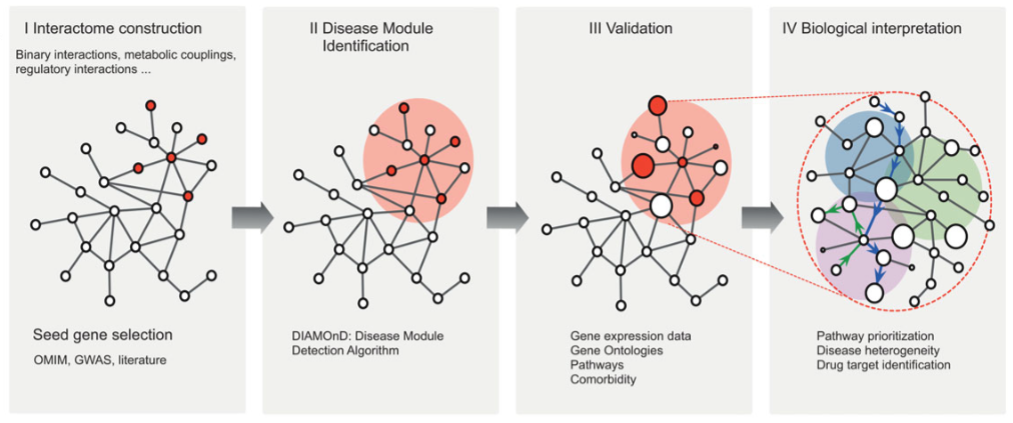
\includegraphics[width=0.5\linewidth]{images/network_module.png}
    \caption{Example of identifying a network module}
    \label{fig:example of a network module}
\end{figure}
    
  \item Most drugs work by binding to one or a few proteins, called the drug's \emph{targets}. A drug whose targets sit close to the disease module is more likely to affect the disease~\cite{guney2016network}.
\begin{figure}[h]
    \centering
    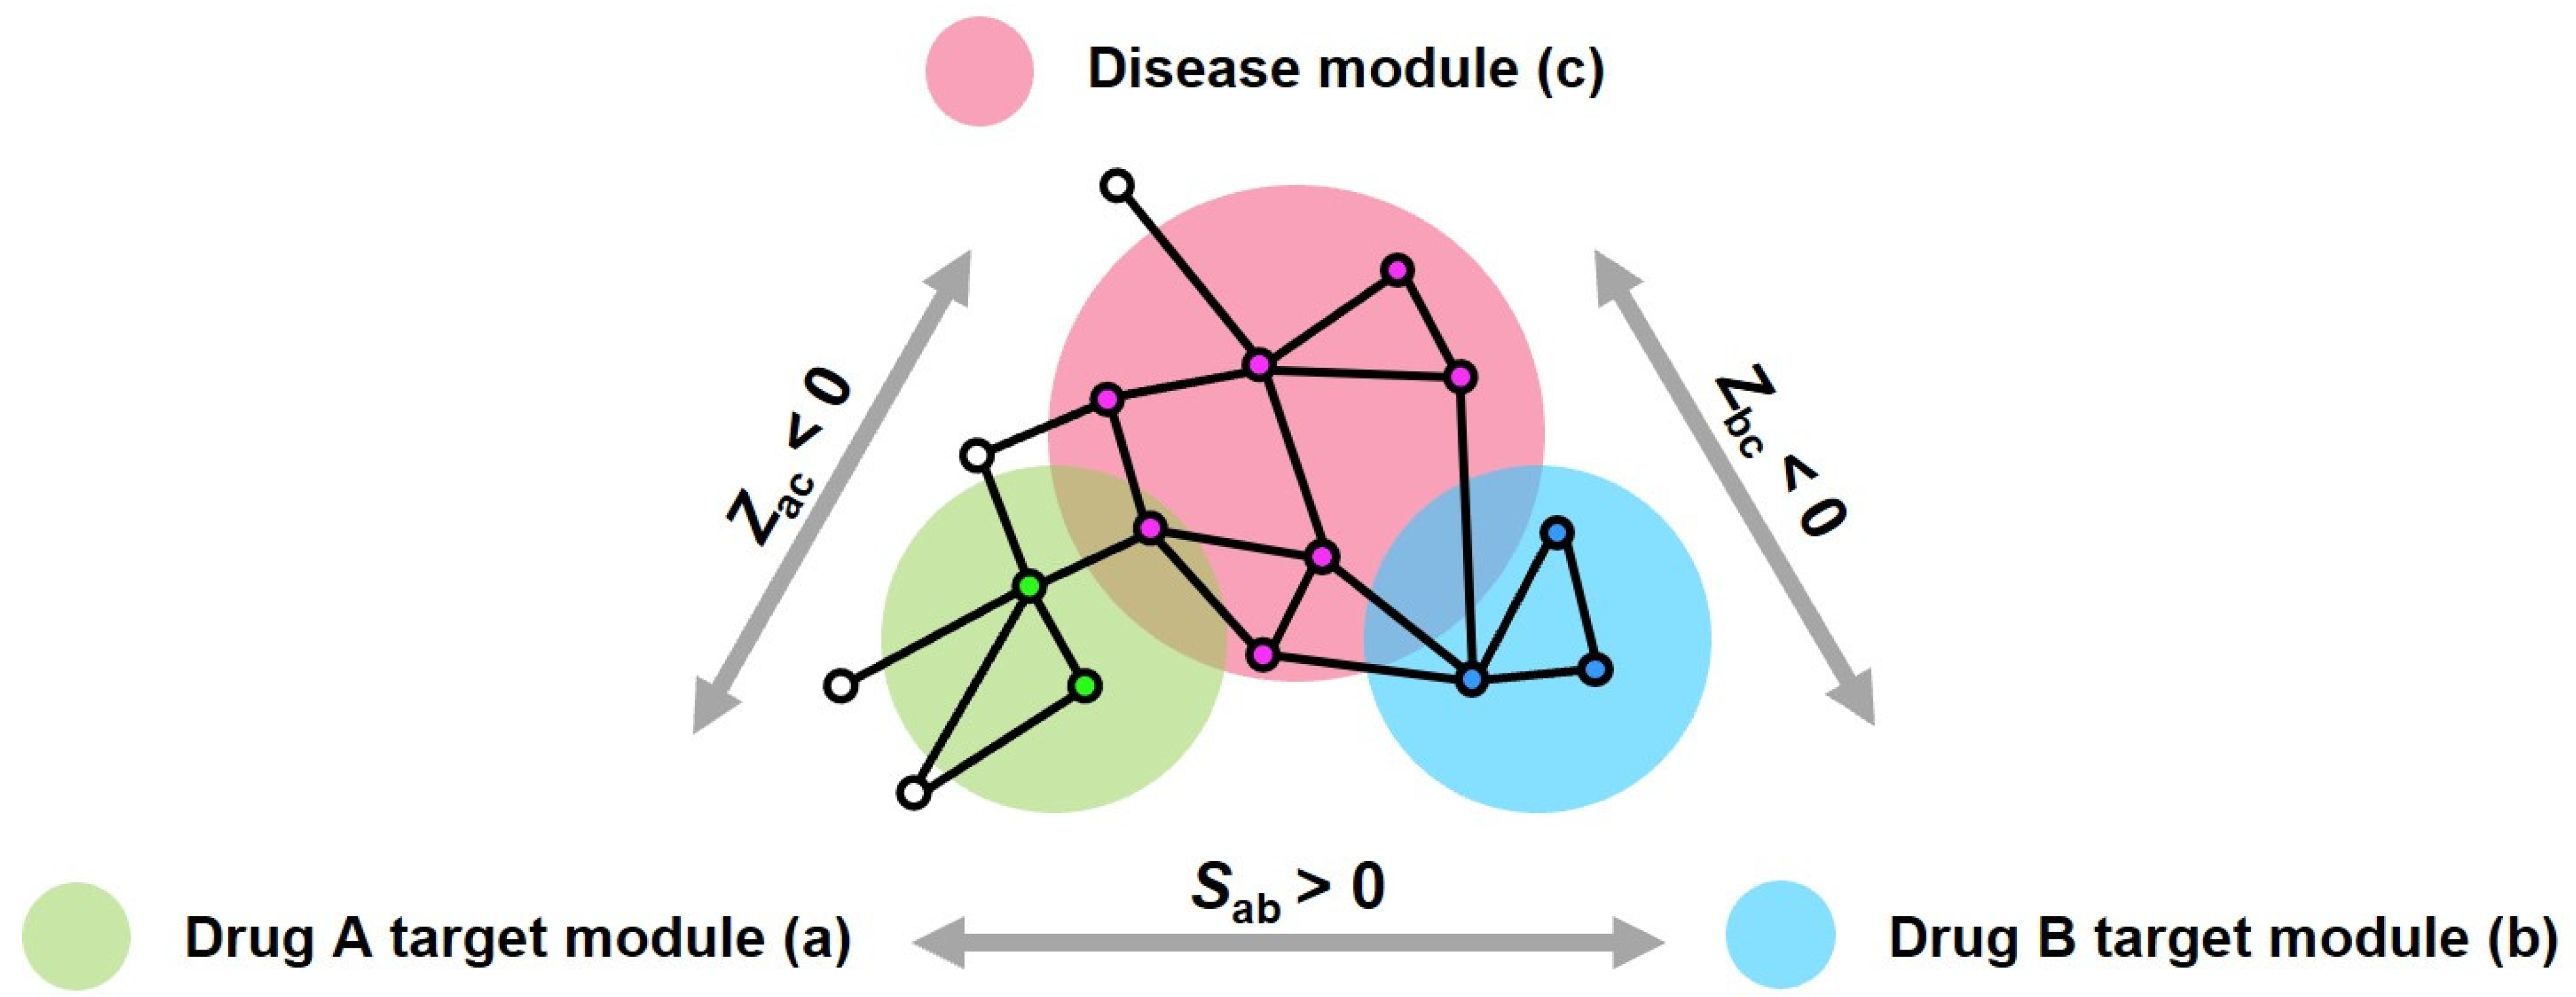
\includegraphics[width=0.5\linewidth]{images/network_drug.png}
    \caption{Example of a drug targeting a disease module}
    \label{fig:enter-label}
\end{figure}
\end{enumerate}

This approach has already produced testable AD hypotheses: network screening combined with analysis of patient insurance records pointed to sildenafil as an AD candidate~\cite{fang2021endophenotype}, and recent pipelines rank drugs for different stages of AD~\cite{csbj2023proximity} or also screen out drugs with heart-rhythm risks~\cite{lqt2025proximity}.

\subsection{Why this is a computer architecture problem}

Distance has to be judged fairly. Hub proteins with many connections are close to almost everything, so a raw distance would favor drugs that simply hit popular proteins. The standard fix~\cite{guney2016network} is to compare each drug against many random ``fake drugs'' whose targets have similar numbers of connections, and report how unusual the real distance is as a $z$-score. This creates a lot of work:
\begin{itemize}[nosep]
  \item shortest-path distances between every pair of proteins: one
        breadth-first search (BFS) from each of $\sim$15{,}000--18{,}000 nodes;
  \item for each of several thousand drugs, 1{,}000 or more random
        samples, each needing many distance look-ups;
  \item for drug combinations, the same distances between every pair of drugs.
\end{itemize}

All of these are \emph{discrete} and \emph{data-parallel}: thousands of independent BFS runs, and millions of independent random samples that each do the same look-up-and-minimum operation. That is exactly the shape of work GPUs are built for. Commonly used tools, however, are single-threaded Python scripts, which limits how many random samples, network versions, and disease modules researchers can afford to test.

\subsection{Supplementary Quantum Computation}

Once single drugs are ranked, a natural next question is which small \emph{combination} of drugs covers the disease module well without the drugs overlapping each other~\cite{cheng2019network}. Choosing the best subset from a shortlist is a yes/no decision per drug, which can be written as a Quadratic Unconstrained Binary Optimization (QUBO) problem~\cite{glover2019tutorial,lucas2014ising}. QUBOs are the standard input for quantum optimization algorithms such as QAOA~\cite{farhi2014qaoa}, which we simulate on the GPU with NVIDIA cuQuantum~\cite{bayraktar2023cuquantum}; no quantum hardware is used. Because the shortlist is small, we can also find the exact best answer by brute force on the GPU and compare QAOA with exact and classical solvers on the same biology-derived problems.

\subsection{What this project delivers}

\begin{enumerate}[nosep]
  \item A CUDA program that computes all shortest-path distances on the human
        interactome and scores every drug's closeness to the AD module.
  \item A sequential C++ version of the same steps, and an
        execution-time comparison between the two.
  \item A ranked list of repurposing candidates for AD, checked against drugs
        that have already entered AD clinical trials.
  \item (Optional) A QUBO formulation of AD drug-combination selection, and a
        benchmark of exact, classical, and GPU-simulated QAOA solvers on it.
\end{enumerate}

Section~\ref{sec:rrl} reviews related work, Section~\ref{sec:problem} states the problem and objectives, and Sections~\ref{sec:method}--\ref{sec:milestones} follow the course outline: project description, target platform, and milestones. Technical details are collected in the appendices.
